\chapter{Probability}

\index{probability}

A \key{probability} is a real number between $0$ and $1$
that indicates how probable an event is.
If an event is certain to happen,
its probability is 1,
and if an event is impossible,
its probability is 0.
The probability of an event is denoted $P(\cdots)$
where the three dots describe the event.

For example, when throwing a dice,
the outcome is an integer between $1$ and $6$,
and it is assumed that the probability of
each outcome is $1/6$.
For example, we can calculate the following probabilities:

\begin{itemize}[noitemsep]
\item $P(\textrm{''the outcome is 4''})=1/6$
\item $P(\textrm{''the outcome is not 6''})=5/6$
\item $P(\textrm{''the outcome is even''})=1/2$
\end{itemize}

\section{Calculation}

To calculate the probability of an event,
we can either use combinatorics
or simulate the process that generates the event.
As an example, let us calculate the probability
of drawing three cards with the same value
from a shuffled deck of cards
(for example, $\spadesuit 8$, $\clubsuit 8$ and $\diamondsuit 8$).

\subsubsection*{Method 1}

We can calculate the probability using the formula

\[\frac{\textrm{number of desired outcomes}}{\textrm{total number of outcomes}}.\]

In this problem, the desired outcomes are those
in which the value of each card is the same.
There are $13 {4 \choose 3}$ such outcomes,
because there are $13$ possibilities for the
value of the cards and ${4 \choose 3}$ ways to
choose $3$ suits from $4$ possible suits.

There are a total of ${52 \choose 3}$ outcomes,
because we choose 3 cards from 52 cards.
Thus, the probability of the event is

\[\frac{13 {4 \choose 3}}{{52 \choose 3}} = \frac{1}{425}.\]

\subsubsection*{Method 2}

Another way to calculate the probability is
to simulate the process that generates the event.
In this case, we draw three cards, so the process
consists of three steps.
We require that each step in the process is successful.

Drawing the first card certainly succeeds,
because there are no restrictions.
The second step succeeds with probability $3/51$,
because there are 51 cards left and 3 of them
have the same value as the first card.
In a similar way, the third step succeeds with probability $2/50$.

The probability that the entire process succeeds is

\[1 \cdot \frac{3}{51} \cdot \frac{2}{50} = \frac{1}{425}.\]

\section{Events}

An event in probability can be represented as a set
\[A \subset X,\]
where $X$ contains all possible outcomes
and $A$ is a subset of outcomes.
For example, when drawing a dice, the outcomes are
\[X = \{1,2,3,4,5,6\}.\]
Now, for example, the event ''the outcome is even''
corresponds to the set
\[A = \{2,4,6\}.\]

Each outcome $x$ is assigned a probability $p(x)$.
Furthermore, the probability $P(A)$ of an event
that corresponds to a set $A$ can be calculated as a sum
of probabilities of outcomes using the formula
\[P(A) = \sum_{x \in A} p(x).\]
For example, when throwing a dice,
$p(x)=1/6$ for each outcome $x$,
so the probability of the event
''the outcome is even'' is
\[p(2)+p(4)+p(6)=1/2.\]

The total probability of the outcomes in $X$ must
be 1, i.e., $P(X)=1$.

Since the events in probability are sets,
we can manipulate them using standard set operations:

\begin{itemize}
\item The \key{complement} $\bar A$ means
''$A$ does not happen''.
For example, when throwing a dice, 
the complement of $A=\{2,4,6\}$ is
$\bar A = \{1,3,5\}$.
\item The \key{union} $A \cup B$ means
''$A$ or $B$ happen''.
For example, the union of
$A=\{2,5\}$
and $B=\{4,5,6\}$ is
$A \cup B = \{2,4,5,6\}$.
\item The \key{intersection} $A \cap B$ means
''$A$ and $B$ happen''.
For example, the intersection of
$A=\{2,5\}$ and $B=\{4,5,6\}$ is
$A \cap B = \{5\}$.
\end{itemize}

\subsubsection{Complement}

The probability of the complement
$\bar A$ is calculated using the formula
\[P(\bar A)=1-P(A).\]

Sometimes, we can solve a problem easily
using complements by solving the opposite problem.
For example, the probability of getting
at least one six when throwing a dice ten times is
\[1-(5/6)^{10}.\]

Here $5/6$ is the probability that the outcome
of a single throw is not six, and
$(5/6)^{10}$ is the probability that none of
the ten throws is a six.
The complement of this is the answer to the problem.

\subsubsection{Union}

The probability of the union $A \cup B$
is calculated using the formula
\[P(A \cup B)=P(A)+P(B)-P(A \cap B).\]
For example, when throwing a dice,
the union of the events
\[A=\textrm{''the outcome is even''}\]
and
\[B=\textrm{''the outcome is less than 4''}\]
is
\[A \cup B=\textrm{''the outcome is even or less than 4''},\]
and its probability is
\[P(A \cup B) = P(A)+P(B)-P(A \cap B)=1/2+1/2-1/6=5/6.\]

If the events $A$ and $B$ are \key{disjoint}, i.e.,
$A \cap B$ is empty,
the probability of the event $A \cup B$ is simply

\[P(A \cup B)=P(A)+P(B).\]

\subsubsection{Conditional probability}

\index{conditional probability}

The \key{conditional probability}
\[P(A | B) = \frac{P(A \cap B)}{P(B)}\]
is the probability of $A$
assuming that $B$ happens.
In this situation, when calculating the
probability of $A$, we only consider the outcomes
that also belong to $B$.

Using the above sets,
\[P(A | B)= 1/3,\]
because the outcomes of $B$ are
$\{1,2,3\}$, and one of them is even.
This is the probability of an even outcome
if we know that the outcome is between $1 \ldots 3$.

\subsubsection{Intersection}

\index{independence}

Using conditional probability,
the probability of the intersection
$A \cap B$ can be calculated using the formula
\[P(A \cap B)=P(A)P(B|A).\]
Events $A$ and $B$ are \key{independent} if
\[P(A|B)=P(A) \hspace{10px}\textrm{and}\hspace{10px} P(B|A)=P(B),\]
which means that the fact that $B$ happens does not
change the probability of $A$, and vice versa.
In this case, the probability of the intersection is
\[P(A \cap B)=P(A)P(B).\]
For example, when drawing a card from a deck, the events
\[A = \textrm{''the suit is clubs''}\]
and
\[B = \textrm{''the value is four''}\]
are independent. Hence the event
\[A \cap B = \textrm{''the card is the four of clubs''}\]
happens with probability
\[P(A \cap B)=P(A)P(B)=1/4 \cdot 1/13 = 1/52.\]

\section{Random variables}

\index{random variable}

A \key{random variable} is a value that is generated
by a random process.
For example, when throwing two dice,
a possible random variable is
\[X=\textrm{''the sum of the outcomes''}.\]
For example, if the outcomes are $[4,6]$
(meaning that we first throw a four and then a six),
then the value of $X$ is 10.

We denote $P(X=x)$ the probability that
the value of a random variable $X$ is $x$.
For example, when throwing two dice,
$P(X=10)=3/36$,
because the total number of outcomes is 36
and there are three possible ways to obtain
the sum 10: $[4,6]$, $[5,5]$ and $[6,4]$.

\subsubsection{Expected value}

\index{expected value}

The \key{expected value} $E[X]$ indicates the
average value of a random variable $X$.
The expected value can be calculated as the sum
\[\sum_x P(X=x)x,\]
where $x$ goes through all possible values of $X$.

For example, when throwing a dice,
the expected outcome is
\[1/6 \cdot 1 + 1/6 \cdot 2 + 1/6 \cdot 3 + 1/6 \cdot 4 + 1/6 \cdot 5 + 1/6 \cdot 6 = 7/2.\]

A useful property of expected values is \key{linearity}.
It means that the sum
$E[X_1+X_2+\cdots+X_n]$
always equals the sum
$E[X_1]+E[X_2]+\cdots+E[X_n]$.
This formula holds even if random variables
depend on each other.

For example, when throwing two dice,
the expected sum is
\[E[X_1+X_2]=E[X_1]+E[X_2]=7/2+7/2=7.\]

Let us now consider a problem where
$n$ balls are randomly placed in $n$ boxes,
and our task is to calculate the expected
number of empty boxes.
Each ball has an equal probability to
be placed in any of the boxes.
For example, if $n=2$, the possibilities
are as follows:
\begin{center}
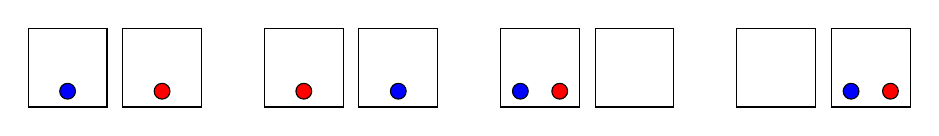
\begin{tikzpicture}
\draw (0,0) rectangle (1,1);
\draw (1.2,0) rectangle (2.2,1);
\draw (3,0) rectangle (4,1);
\draw (4.2,0) rectangle (5.2,1);
\draw (6,0) rectangle (7,1);
\draw (7.2,0) rectangle (8.2,1);
\draw (9,0) rectangle (10,1);
\draw (10.2,0) rectangle (11.2,1);

\draw[fill=blue] (0.5,0.2) circle (0.1);
\draw[fill=red] (1.7,0.2) circle (0.1);
\draw[fill=red] (3.5,0.2) circle (0.1);
\draw[fill=blue] (4.7,0.2) circle (0.1);
\draw[fill=blue] (6.25,0.2) circle (0.1);
\draw[fill=red] (6.75,0.2) circle (0.1);
\draw[fill=blue] (10.45,0.2) circle (0.1);
\draw[fill=red] (10.95,0.2) circle (0.1);
\end{tikzpicture}
\end{center}
In this case, the expected number of
empty boxes is
\[\frac{0+0+1+1}{4} = \frac{1}{2}.\]
In the general case, the probability that a
single box is empty is
\[\Big(\frac{n-1}{n}\Big)^n,\]
because no ball should be placed in it.
Hence, using linearity, the expected number of
empty boxes is
\[n \cdot \Big(\frac{n-1}{n}\Big)^n.\]

\subsubsection{Distributions}

\index{distribution}

The \key{distribution} of a random variable $X$
shows the probability of each value that
$X$ may have.
The distribution consists of values $P(X=x)$.
For example, when throwing two dice,
the distribution for their sum is:
\begin{center}
\small {
\begin{tabular}{r|rrrrrrrrrrrrr}
$x$ & 2 & 3 & 4 & 5 & 6 & 7 & 8 & 9 & 10 & 11 & 12 \\
$P(X=x)$ & $1/36$ & $2/36$ & $3/36$ & $4/36$ & $5/36$ & $6/36$ & $5/36$ & $4/36$ & $3/36$ & $2/36$ & $1/36$ \\
\end{tabular}
}
\end{center}

\index{uniform distribution}
In a \key{uniform distribution},
the random variable $X$ has $n$ possible
values $a,a+1,\ldots,b$ and the probability of each value is $1/n$.
For example, when throwing a dice,
$a=1$, $b=6$ and $P(X=x)=1/6$ for each value $x$.

The expected value for $X$ in a uniform distribution is
\[E[X] = \frac{a+b}{2}.\]
\index{binomial distribution}
~\\
In a \key{binomial distribution}, $n$ attempts
are made
and the probability that a single attempt succeeds
is $p$.
The random variable $X$ counts the number of
successful attempts,
and the probability for a value $x$ is
\[P(X=x)=p^x (1-p)^{n-x} {n \choose x},\]
where $p^x$ and $(1-p)^{n-x}$ correspond to
successful and unsuccessful attemps,
and ${n \choose x}$ is the number of ways
we can choose the order of the attempts.

For example, when throwing a dice ten times,
the probability of throwing a six exactly
three times is $(1/6)^3 (5/6)^7 {10 \choose 3}$.

The expected value for $X$ in a binomial distribution is
\[E[X] = pn.\]
\index{geometric distribution}
~\\
In a \key{geometric distribution},
the probability that an attempt succeeds is $p$,
and we continue until the first success happens.
The random variable $X$ counts the number
of attempts needed, and the probability for
a value $x$ is
\[P(X=x)=(1-p)^{x-1} p,\]
where $(1-p)^{x-1}$ corresponds to unsuccessful attemps
and $p$ corresponds to the first successful attempt.

For example, if we throw a dice until we throw a six,
the probability that the number of throws
is exactly 4 is $(5/6)^3 1/6$.

The expected value for $X$ in a geometric distribution is
\[E[X]=\frac{1}{p}.\]

\section{Markov chains}

\index{Markov chain}

A \key{Markov chain}
% \footnote{A. A. Markov (1856--1922)
% was a Russian mathematician.}
is a random process
that consists of states and transitions between them.
For each state, we know the probabilities
for moving to other states.
A Markov chain can be represented as a graph
whose nodes are states and edges are transitions.

As an example, let us consider a problem
where we are in floor 1 in an $n$ floor building.
At each step, we randomly walk either one floor
up or one floor down, except that we always
walk one floor up from floor 1 and one floor down
from floor $n$.
What is the probability of being in floor $m$
after $k$ steps?

In this problem, each floor of the building
corresponds to a state in a Markov chain.
For example, if $n=5$, the graph is as follows:

\begin{center}
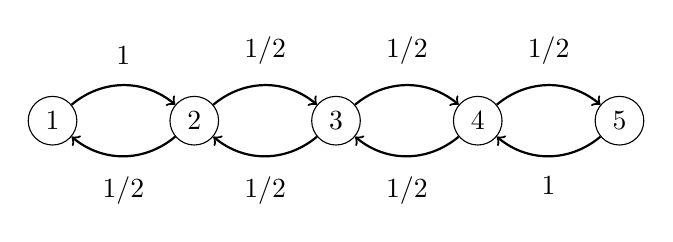
\begin{tikzpicture}[scale=0.9]
\node[draw, circle] (1) at (0,0) {$1$};
\node[draw, circle] (2) at (2,0) {$2$};
\node[draw, circle] (3) at (4,0) {$3$};
\node[draw, circle] (4) at (6,0) {$4$};
\node[draw, circle] (5) at (8,0) {$5$};

\path[draw,thick,->] (1) edge [bend left=40] node[font=\small,label=$1$] {} (2);
\path[draw,thick,->] (2) edge [bend left=40] node[font=\small,label=$1/2$] {} (3);
\path[draw,thick,->] (3) edge [bend left=40] node[font=\small,label=$1/2$] {} (4);
\path[draw,thick,->] (4) edge [bend left=40] node[font=\small,label=$1/2$] {} (5);

\path[draw,thick,->] (5) edge [bend left=40] node[font=\small,label=below:$1$] {} (4);
\path[draw,thick,->] (4) edge [bend left=40] node[font=\small,label=below:$1/2$] {} (3);
\path[draw,thick,->] (3) edge [bend left=40] node[font=\small,label=below:$1/2$] {} (2);
\path[draw,thick,->] (2) edge [bend left=40] node[font=\small,label=below:$1/2$] {} (1);

%\path[draw,thick,->] (1) edge [bend left=40] node[font=\small,label=below:$1$] {} (2);
\end{tikzpicture}
\end{center}

The probability distribution
of a Markov chain is a vector
$[p_1,p_2,\ldots,p_n]$, where $p_k$ is the
probability that the current state is $k$.
The formula $p_1+p_2+\cdots+p_n=1$ always holds.

In the example, the initial distribution is
$[1,0,0,0,0]$, because we always begin in floor 1.
The next distribution is $[0,1,0,0,0]$,
because we can only move from floor 1 to floor 2.
After this, we can either move one floor up
or one floor down, so the next distribution is
$[1/2,0,1/2,0,0]$, and so on.

An efficient way to simulate the walk in
a Markov chain is to use dynamic programming.
The idea is to maintain the probability distribution
and at each step go through all possibilities
how we can move.
Using this method, we can simulate $m$ steps
in $O(n^2 m)$ time.

The transitions of a Markov chain can also be
represented as a matrix that updates the
probability distribution.
In this example, the matrix is

\[ 
 \begin{bmatrix}
  0 & 1/2 & 0 & 0 & 0 \\
  1 & 0 & 1/2 & 0 & 0 \\
  0 & 1/2 & 0 & 1/2 & 0 \\
  0 & 0 & 1/2 & 0 & 1 \\
  0 & 0 & 0 & 1/2 & 0 \\
 \end{bmatrix}.
\]

When we multiply a probability distribution by this matrix,
we get the new distribution after moving one step.
For example, we can move from the distribution
$[1,0,0,0,0]$ to the distribution
$[0,1,0,0,0]$ as follows:

\[ 
 \begin{bmatrix}
  0 & 1/2 & 0 & 0 & 0 \\
  1 & 0 & 1/2 & 0 & 0 \\
  0 & 1/2 & 0 & 1/2 & 0 \\
  0 & 0 & 1/2 & 0 & 1 \\
  0 & 0 & 0 & 1/2 & 0 \\
 \end{bmatrix}
 \begin{bmatrix}
  1 \\
  0 \\
  0 \\
  0 \\
  0 \\
 \end{bmatrix}
=
 \begin{bmatrix}
  0 \\
  1 \\
  0 \\
  0 \\
  0 \\
 \end{bmatrix}.
\]

By calculating matrix powers efficiently,
we can calculate the distribution after $m$ steps
in $O(n^3 \log m)$ time.

\section{Randomized algorithms}

\index{randomized algorithm}

Sometimes we can use randomness for solving a problem,
even if the problem is not related to probabilities.
A \key{randomized algorithm} is an algorithm that
is based on randomness.

\index{Monte Carlo algorithm}

A \key{Monte Carlo algorithm} is a randomized algorithm
that may sometimes give a wrong answer.
For such an algorithm to be useful,
the probability of a wrong answer should be small.

\index{Las Vegas algorithm}

A \key{Las Vegas algorithm} is a randomized algorithm
that always gives the correct answer,
but its running time varies randomly.
The goal is to design an algorithm that is
efficient with high probability.

Next we will go through three example problems that
can be solved using randomness.

\subsubsection{Order statistics}

\index{order statistic}

The $kth$ \key{order statistic} of an array
is the element at position $k$ after sorting
the array in increasing order.
It is easy to calculate any order statistic
in $O(n \log n)$ time by sorting the array,
but is it really needed to sort the entire array
just to find one element?

It turns out that we can find order statistics
using a randomized algorithm without sorting the array.
The algorithm, called \key{quickselect}\footnote{In 1961,
C. A. R. Hoare published two algorithms that
are efficient on average: \index{quicksort} \index{quickselect}
\key{quicksort} \cite{hoa61a} for sorting arrays and
\key{quickselect} \cite{hoa61b} for finding order statistics.}, is a Las Vegas algorithm:
its running time is usually $O(n)$
but $O(n^2)$ in the worst case.

The algorithm chooses a random element $x$
in the array, and moves elements smaller than $x$
to the left part of the array,
and all other elements to the right part of the array.
This takes $O(n)$ time when there are $n$ elements.
Assume that the left part contains $a$ elements
and the right part contains $b$ elements.
If $a=k-1$, element $x$ is the $k$th order statistic.
Otherwise, if $a>k-1$, we recursively find the $k$th order
statistic for the left part,
and if $a<k-1$, we recursively find the $r$th order
statistic for the right part where $r=k-a$.
The search continues in a similar way, until the element
has been found.

When each element $x$ is randomly chosen,
the size of the array about halves at each step,
so the time complexity for
finding the $k$th order statistic is about
\[n+n/2+n/4+n/8+\cdots=O(n).\]

The worst case for the algorithm is still $O(n^2)$,
because it is possible that $x$ is always chosen
in such a way that it is one of the smallest or largest
elements in the array and $O(n)$ steps are needed.
However, the probability for this is so small
that this never happens in practice.

\subsubsection{Verifying matrix multiplication}

\index{matrix multiplication}

Our next problem is to \emph{verify}
if $AB=C$ holds when $A$, $B$ and $C$
are matrices of size $n \times n$.
Of course, we can solve the problem
by calculating the product $AB$ again
(in $O(n^3)$ time using the basic algorithm),
but one could hope that verifying the
answer would by easier than to calculate it from scratch.

It turns out that we can solve the problem
using a Monte Carlo algorithm\footnote{R. M. Freivalds published
this algorithm in 1977 \cite{fre77}, and it is sometimes
called \index{Freivalds' algoritm} \key{Freivalds' algorithm}.} whose
time complexity is only $O(n^2)$.
The idea is simple: we choose a random vector
$X$ of $n$ elements, and calculate the matrices
$ABX$ and $CX$. If $ABX=CX$, we report that $AB=C$,
and otherwise we report that $AB \neq C$.

The time complexity of the algorithm is
$O(n^2)$, because we can calculate the matrices
$ABX$ and $CX$ in $O(n^2)$ time.
We can calculate the matrix $ABX$ efficiently
by using the representation $A(BX)$, so only two
multiplications of $n \times n$ and $n \times 1$
size matrices are needed.

The drawback of the algorithm is
that there is a small chance that the algorithm
makes a mistake when it reports that $AB=C$.
For example, 
\[
 \begin{bmatrix}
  2 & 4 \\
  1 & 6 \\
 \end{bmatrix}
\neq
 \begin{bmatrix}
  0 & 5 \\
  7 & 4 \\
 \end{bmatrix},
\]
but
\[
 \begin{bmatrix}
  2 & 4 \\
  1 & 6 \\
 \end{bmatrix}
 \begin{bmatrix}
  1 \\
  3 \\
 \end{bmatrix}
=
 \begin{bmatrix}
  0 & 5 \\
  7 & 4 \\
 \end{bmatrix}
 \begin{bmatrix}
  1 \\
  3 \\
 \end{bmatrix}.
\]
However, in practice, the probability that the
algorithm makes a mistake is small,
and we can decrease the probability by
verifying the result using multiple random vectors $X$
before reporting that $AB=C$.

\subsubsection{Graph coloring}

\index{coloring}

Given a graph that contains $n$ nodes and $m$ edges,
our task is to find a way to color the nodes
of the graph using two colors so that
for at least $m/2$ edges, the endpoints 
have different colors.
For example, in the graph
\begin{center}
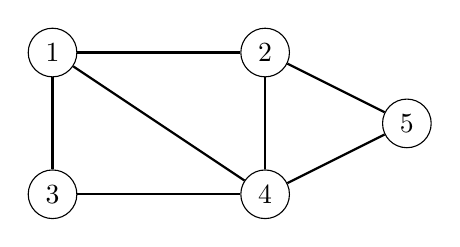
\begin{tikzpicture}[scale=0.9]
\node[draw, circle] (1) at (1,3) {$1$};
\node[draw, circle] (2) at (4,3) {$2$};
\node[draw, circle] (3) at (1,1) {$3$};
\node[draw, circle] (4) at (4,1) {$4$};
\node[draw, circle] (5) at (6,2) {$5$};

\path[draw,thick,-] (1) -- (2);
\path[draw,thick,-] (1) -- (3);
\path[draw,thick,-] (1) -- (4);
\path[draw,thick,-] (3) -- (4);
\path[draw,thick,-] (2) -- (4);
\path[draw,thick,-] (2) -- (5);
\path[draw,thick,-] (4) -- (5);
\end{tikzpicture}
\end{center}
a valid coloring is as follows:
\begin{center}
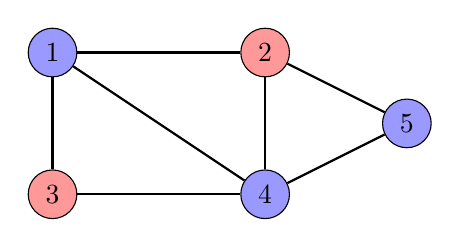
\begin{tikzpicture}[scale=0.9]
\node[draw, circle, fill=blue!40] (1) at (1,3) {$1$};
\node[draw, circle, fill=red!40] (2) at (4,3) {$2$};
\node[draw, circle, fill=red!40] (3) at (1,1) {$3$};
\node[draw, circle, fill=blue!40] (4) at (4,1) {$4$};
\node[draw, circle, fill=blue!40] (5) at (6,2) {$5$};

\path[draw,thick,-] (1) -- (2);
\path[draw,thick,-] (1) -- (3);
\path[draw,thick,-] (1) -- (4);
\path[draw,thick,-] (3) -- (4);
\path[draw,thick,-] (2) -- (4);
\path[draw,thick,-] (2) -- (5);
\path[draw,thick,-] (4) -- (5);
\end{tikzpicture}
\end{center}
The above graph contains 7 edges, and for 5 of them,
the endpoints have different colors,
so the coloring is valid.

The problem can be solved using a Las Vegas algorithm
that generates random colorings until a valid coloring
has been found.
In a random coloring, the color of each node is
independently chosen so that the probability of
both colors is $1/2$.

In a random coloring, the probability that the endpoints
of a single edge have different colors is $1/2$.
Hence, the expected number of edges whose endpoints
have different colors is $m/2$.
Since it is excepted that a random coloring is valid,
we will quickly find a valid coloring in practice.

